\section{Symulacje układów}
    \begin{figure}[!ht]
        \centering
        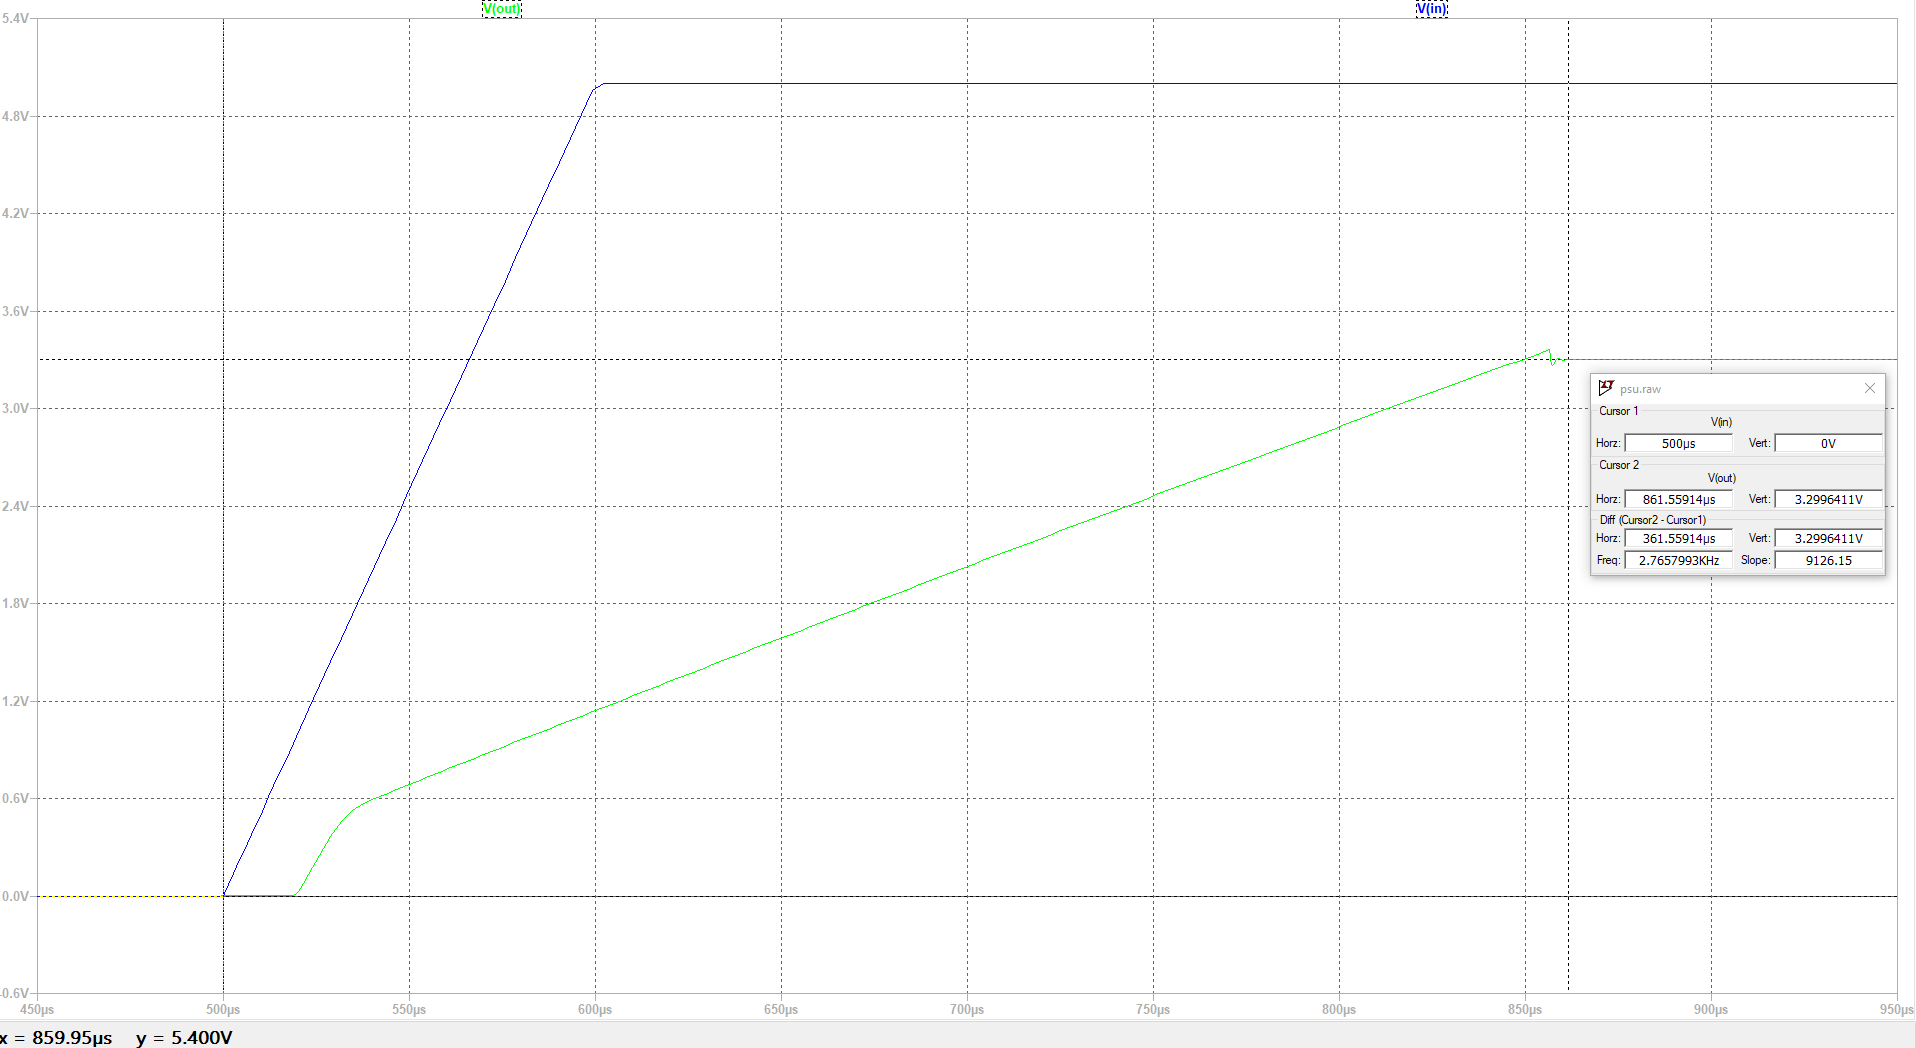
\includegraphics[width=\textwidth]{psu_tran.png}
        \caption{Symulacja tran stabilizatora napięcia LM1117-3.3 napięcia wejściowego ($V_{in}$) i wyjściowego ($V_{out}$).}
        \label{fig:sym_LM1117}
    \end{figure}
    \begin{figure}[!ht]
        \centering
        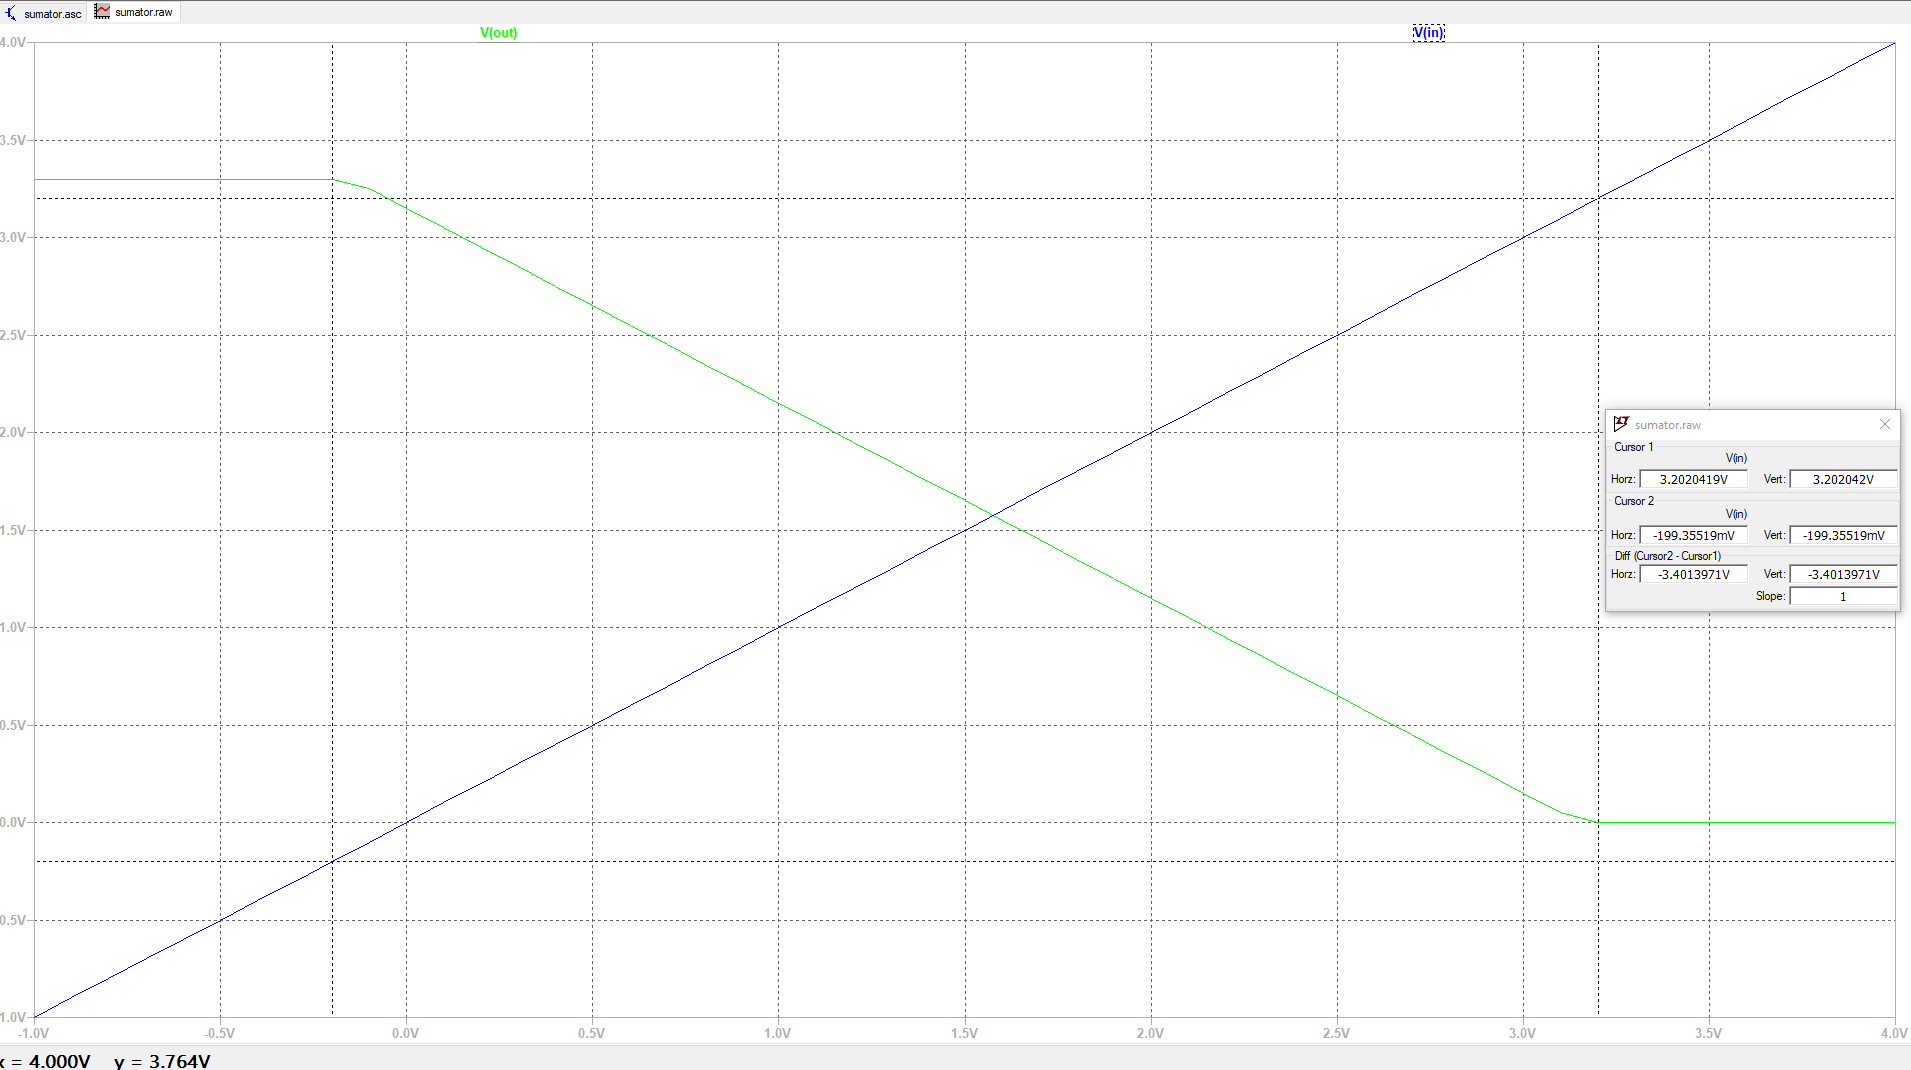
\includegraphics[width=\textwidth]{sumator_dc.png}
        \caption{Symulacja dc układu sumującego, napięcia wyjściowego ($V_{out}$) od napięcia wejściowego ($V_{in}$).}
        \label{fig:sym_sum}
    \end{figure}
    \begin{figure}[!ht]
        \centering
        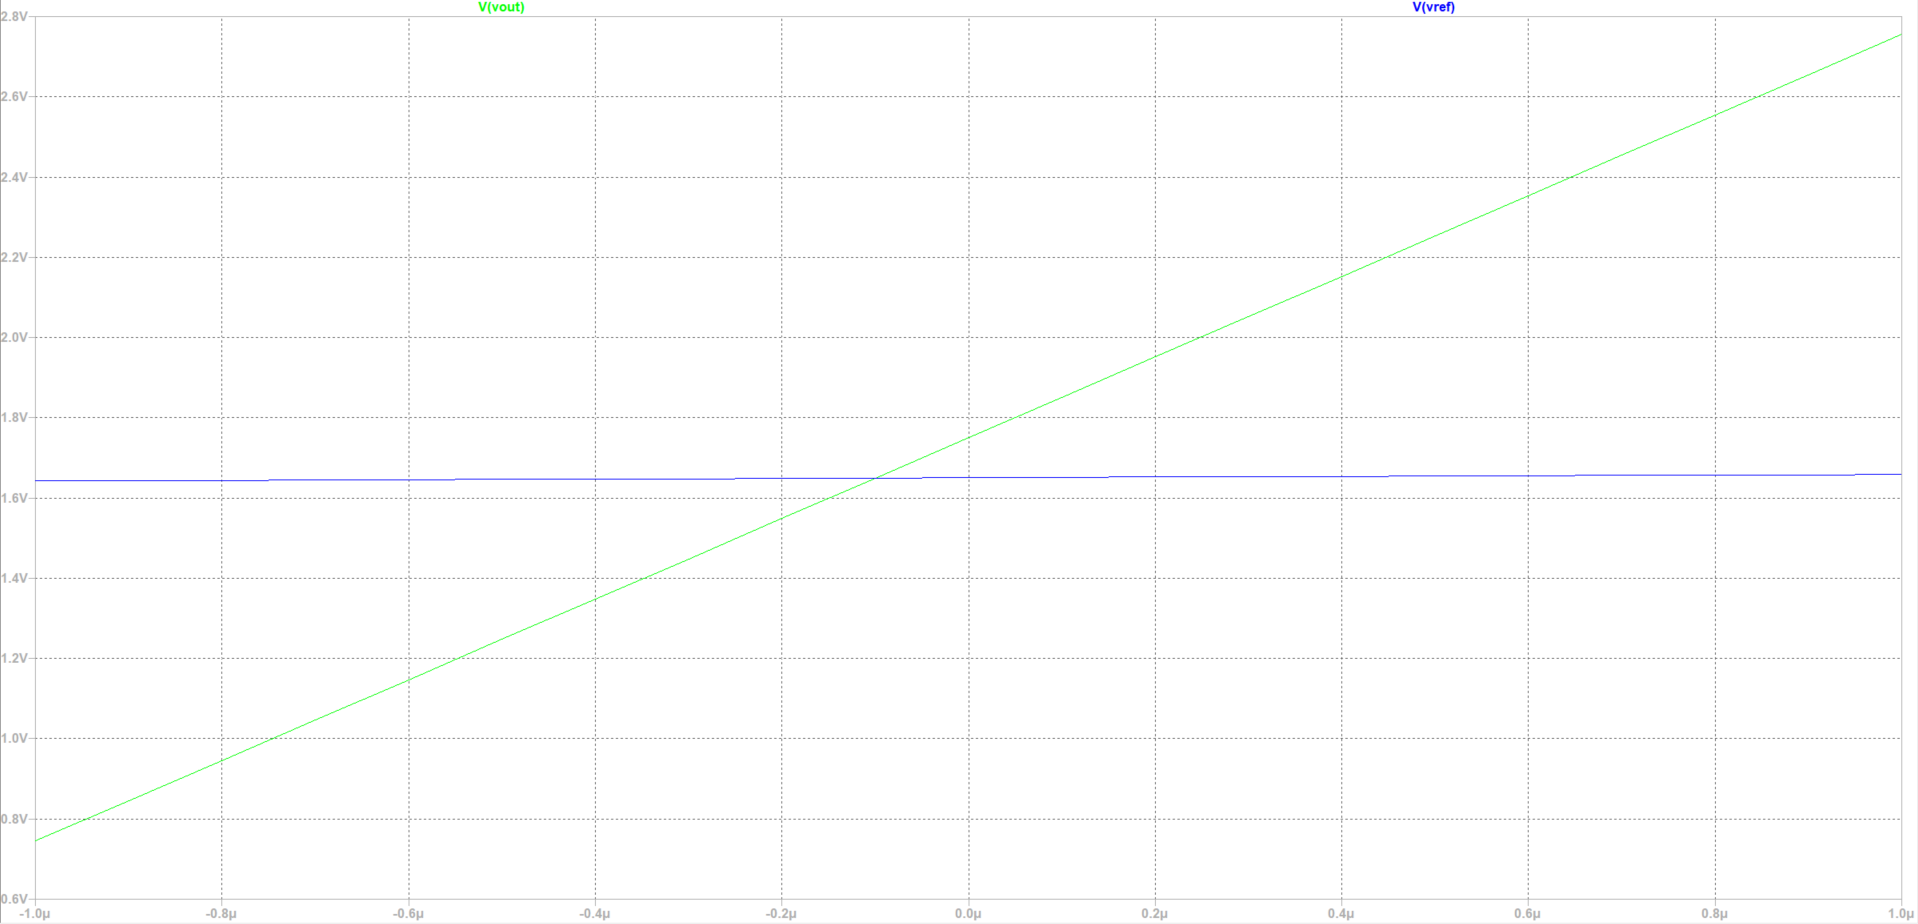
\includegraphics[width=\textwidth]{INA333_1u_range.png}
        \caption{Symulacja parametryczna wzmacniacza pomiarowego w zakresie $\pm 1\ \mu A$.}
        \label{fig:sym_INA_1u}
    \end{figure}
    \begin{figure}[!ht]
        \centering
        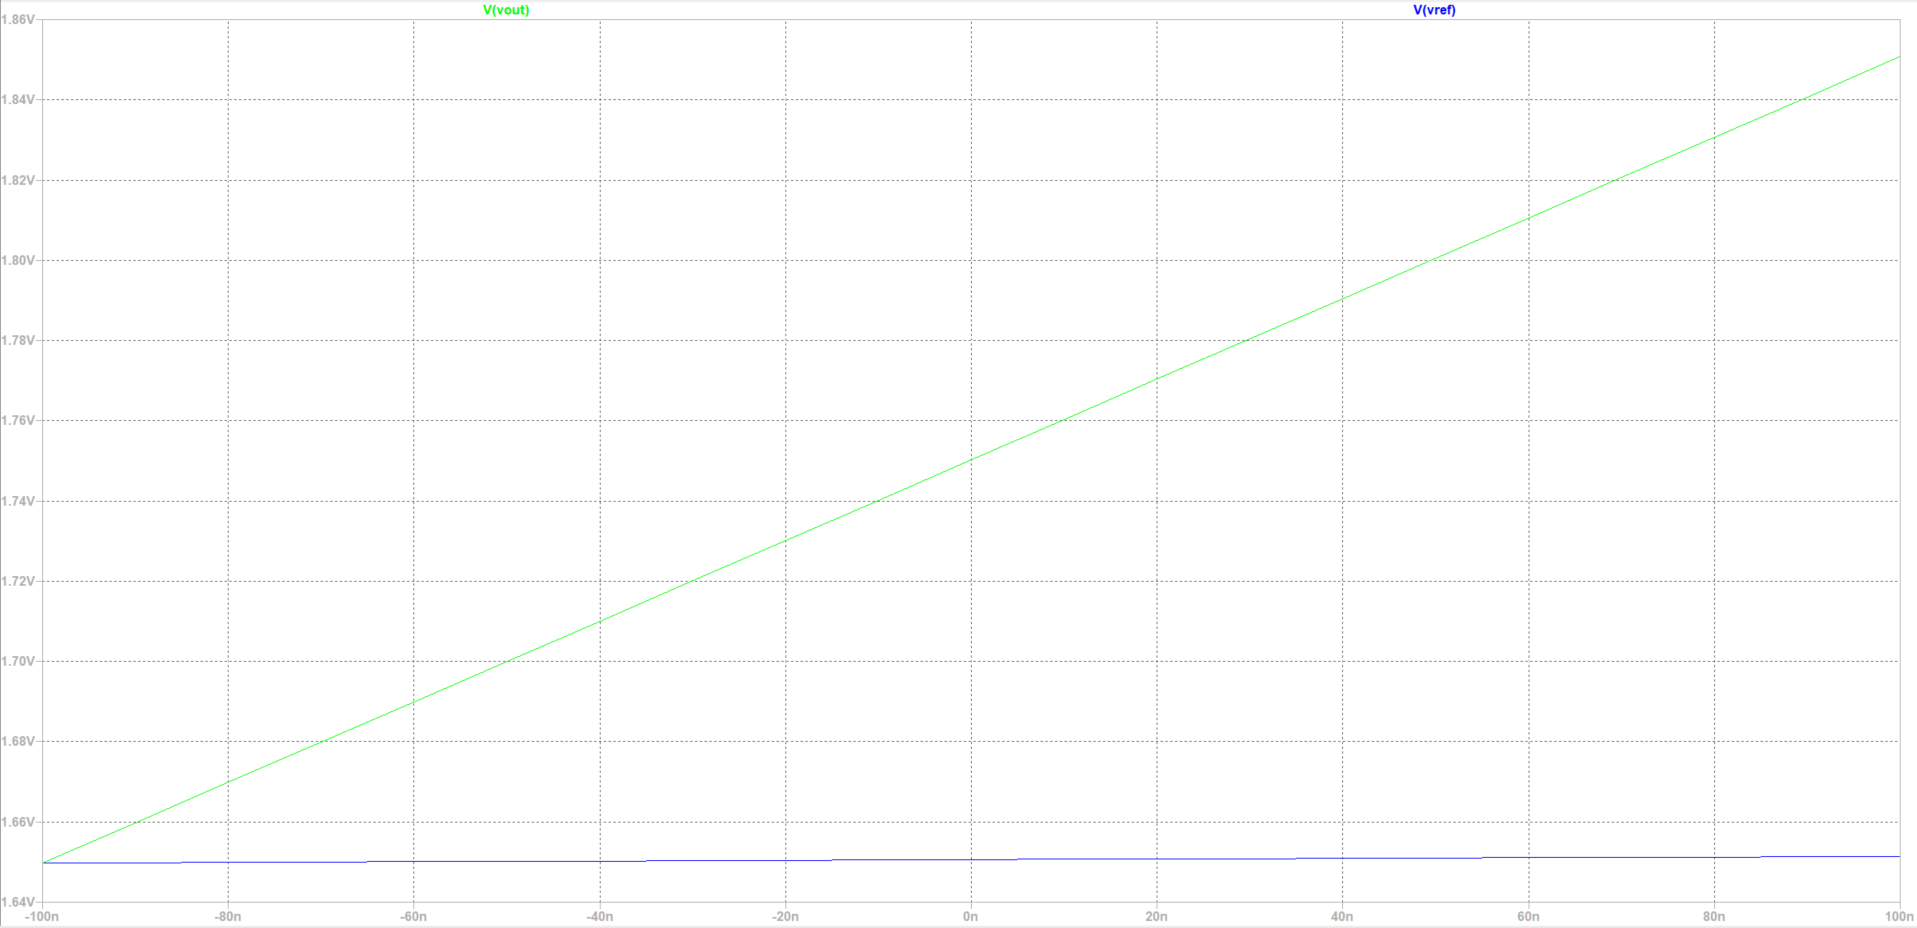
\includegraphics[width=\textwidth]{INA333_100n_range.png}
        \caption{Symulacja parametryczna wzmacniacza pomiarowego w zakresie $\pm 100\ nA$.}
        \label{fig:sym_INA_100n}
    \end{figure}
